\subsection{Definition of TMDs}
\label{sec:tmd_definition}
Consider a frame of reference where the nucleon has large momentum in the $z$-direction, i.e., $P^+ \gg m_N$, $\vprp{P} = 0$.
In light cone coordinates, the components $\kei^+$,~$\vprp{\kei}$,~$\kei^-$ of the quark momentum $\kei$ scale as $P^+/m_N$,~$1$,~$m_N/P^+$, respectively, under boosts along the $z$-axis. Thus, the quark longitudinal momentum fraction $x = k^+ / P^+$ and the transverse momentum $\vprp{\kei}$ are invariant under boosts along the $z$-axis, while the $k^-$ component is suppressed. 
This leads to transverse momentum-dependent parton distribution functions (TMDs), which depend on the longitudinal momentum fraction $x \equiv \kei^+ / P^+$ and the quark transverse momentum $\vprp{\kei}$. 
The transverse momentum components $\vprp{\kei}$ describe an intrinsic motion of the quarks inside the proton that occurs independently of the momentum of the proton itself. TMDs are an important ingredient for understanding the origin of the large angular and spin asymmetries observed in experiments such as semi-inclusive deep inelastic scattering (SIDIS) and the Drell-Yan process (DY).

We construct a correlator from the gauge-invariant bilocal operator $\bar q(0) \Gamma \WlineC{\mathcal{C}_\bvec} q(\bvec)$ acting on the nucleon state $\ket{P, S}$, where $\bar q$ and $q$ are local quark field operators, and the Wilson line $\WlineC{\mathcal{C}_\bvec}$ makes the bi-local operator gauge invariant. The Fourier transform of such a position space correlator $\bra{P,S}\ \bar{q}(0)\, \Gamma\ \WlineC{\mathcal{C}_\bvec}\ q(\bvec)\ \ket{P,S}$ with respect to $b$ gives the momentum space correlator $\Phi^{[\Gamma]}(\kei,P,S;\ldots)$, or equivalently the TMDs. The Wilson
line (to be specified in more detail below) introduces divergences that conventional dimensional
regularization cannot treat~\cite{Musch:2011er}, so we divide by the soft factor, $\widetilde{\softf}(\bvec^2;\ldots)$, 
\begin{widetext}
\begin{align}
	\Phi^{[\Gamma]}(\kei,P,S;\ldots)\ \equiv\ \ 
	\int \frac{d^4 \bvec}{(2\pi)^4}\, e^{i \kei\cdot \bvec}\,
		\frac{\overbrace{\rule{0em}{1.2em}
		\frac{1}{2}\, \bra{P,S}\ \bar{q}(0)\, \Gamma\ \WlineC{\mathcal{C}_\bvec}\ q(\bvec)\ \ket{P,S}
		}^{\displaystyle \equiv \widetilde \Phi_\unsub^{[\Gamma]}(\bvec,P,S;\ldots)}}
		{ \widetilde{\softf}(\bvec^2;\ldots) } \ .
		\label{eq-corr}	
\end{align}
\end{widetext}
The numerator, $\widetilde \Phi_\unsub^{[\Gamma]}(\bvec, P,S;\ldots)$, is the bare non-local matrix element in which a gauge link $\WlineC{\mathcal{C}_\bvec}$ connects the quark fields. The denominator is the soft factor, $\widetilde{\softf}(\bvec^2;\ldots)$, which regulates rapidity divergences. The ellipses (``$\ldots$'') denote additional dependence on parameters governing the Wilson line geometry and the soft factor, as well as an implicit dependence on the ultraviolet renormalization scale $\mu$.

The soft factor, $\tilde \softf$, stands symbolically for an
expression that can, depending on the formalism, involve several vacuum
expectation values. In the framework of Collins and Aybat~\cite{Aybat:2011zv,CollinsBook2011,Aybat:2011ge}, it takes the form
\begin{equation}
\widetilde{\softf}(\bvec^2;\ldots) = 
  \sqrt{ \frac
    { \tilde S_{(0)}( \vprp{\bvec}, + \infty, -\infty )\ \tilde S_{(0)}( \vprp{\bvec}, y_s, -\infty ) }
    { \tilde S_{(0)}( \vprp{\bvec}, + \infty, y_s ) }
  } \ ,
\end{equation}
here each of the objects $\tilde S_{(0)}( \vprp{\bvec}, \ldots )$ is a
vacuum expectation value of Wilson line structures.
In this framework, we start with space-like Wilson lines. Some Wilson lines remain tilted away from the light cone, leading to the dependence on the rapidity parameter $y_s$ in the above expression. We need not specify $\tilde \softf$ further, since it cancels in the observables we consider.

To project the correlator onto the relevant kinematics, we integrate over the suppressed momentum component $k^-$, which sets the position-space separation to $b^+ = 0$:
\begin{widetext}
\begin{align}
	\Phi^{[\Gamma]}(x,\vprp{k};P,S;\ldots) & \equiv \int dk^{-} \Phi^{[\Gamma]}(\kei,P,S;\ldots) \nonumber \\ 
 &=\int dk^{-}\int \frac{d^4 \bvec}{(2\pi)^4}\, e^{i \kei\cdot \bvec} \frac{\frac{1}{2}\, \bra{P,S}\ \bar{q}(0)\, \Gamma\ \WlineC{\mathcal{C}_\bvec}\ q(\bvec)\ \ket{P,S}}{ \widetilde{\mathcal{S}}(-\vprp{\bvec}^2;\ldots) }\\
 &=\int dk^{-}\int \frac{db^{+}}{2\pi}e^{ik^-b^+}\int \frac{d^2\textbf{b}_T}{(2\pi)^2}\int \frac{db^-}{2\pi}e^{ik^+b^--i\textbf{k}_T\tcdot\textbf{b}_T}\frac{\frac{1}{2}\, \bra{P,S}\ \bar{q}(0)\, \Gamma\ \WlineC{\mathcal{C}_\bvec}\ q(\bvec)\ \ket{P,S}}{ \widetilde{\mathcal{S}}(-\vprp{\bvec}^2;\ldots) }\\
 &=\int {db^{+}}\delta(b^+)\int \frac{d^2\textbf{b}_T}{(2\pi)^2}\int \frac{db^-}{2\pi}e^{ik^+b^--i\textbf{k}_T\tcdot\textbf{b}_T}\frac{\frac{1}{2}\, \bra{P,S}\ \bar{q}(0)\, \Gamma\ \WlineC{\mathcal{C}_\bvec}\ q(\bvec)\ \ket{P,S}}{ \widetilde{\mathcal{S}}(-\vprp{\bvec}^2;\ldots) }\\
	& =\int \frac{d^2 \vprp{\bvec}}{(2\pi)^2} \int \frac{d (\bvec \tcdot P)}{(2\pi) P^+}\ e^{i x (\bvec \tcdot P) - i\vprp{\bvec} \tcdot \vprp{\kei}}\,
		\left. \frac{\frac{1}{2}\, \bra{P,S}\ \bar{q}(0)\, \Gamma\ \WlineC{\mathcal{C}_\bvec}\ q(\bvec)\ \ket{P,S}}
		{ \widetilde{\mathcal{S}}(-\vprp{\bvec}^2;\ldots) } \right|_{b^+ = 0} \ .
\end{align}
\end{widetext}
As a consequence, $x \leftrightarrow (\bvec \tcdot P)$ and $\vprp{k} \leftrightarrow \vprp{b}$ are independent pairs of Fourier conjugate variables.
With the Dirac matrix $\Gamma = \gamma^+$, which projects onto the leading-twist unpolarized quark distribution, the correlator becomes~\cite{Ralston:1979ys, Tangerman:1994eh,Mulders:1995dh,Goeke:2005hb}:
\begin{align}
	\Phi^{[\gamma^+]}(x,\vprp{k};P,S,\ldots) & = f_1 - \toddmark{\frac{\myeps_{ij}\, \vect{k}_{i}\, \vect{S}_{j}}{m_N}\ f_{1T}^\prp} \label{eq-phigammaplus}\ . 
\end{align}
The term enclosed in $[\ ]_\text{odd}$ isolates the naively time-reversal odd (T-odd) Sivers function $f_{1T}^\perp$~\cite{Sivers:1989cc}, which describes the distribution of unpolarized quarks inside a transversely polarized nucleon. The origin of this parametrization and the special role of T-odd TMDs become clear once we discuss the geometry of the gauge link path $\mathcal{C}_\bvec $ and symmetry transformation properties.
\subsection{TMDs in Fourier space}
\label{sec:tmd_fourier}
Our lattice method evaluates the $b$-dependent matrix elements $\widetilde \Phi_\unsub^{[\Gamma]}(\bvec,P,S;\ldots)$ introduced in Eq. \eqref{eq-corr}. It is therefore more direct and natural to state our results in terms of Fourier-transformed, $\vprp{b}$-dependent TMDs and their $\vprp{b}$-derivatives. For a generic TMD $f$, we define the Fourier transform and its derivatives:
\begin{widetext}
\begin{align}
	\tilde f(x, \vprp{\bvec}^2;\ldots) & \equiv \int  d^2 \vprp{\kei} \, e^{i \vprp{\bvec} \cdot \vprp{\kei} }\; f(x, \vprp{\kei}^2;\ldots)
		= 2\pi \int      d|\vprp{\kei}| |\vprp{\kei}|\ J_0(|\vprp{\bvec}||\vprp{\kei}|)\  f(x, {\vprp{\kei}^2};\ldots )\ , \label{eq-FTMD} \\
	\tilde f^{(n)}(x, \vprp{\bvec}^2\ldots ) & \equiv n!\left( -\frac{2}{\mN^2}\partial_{\vprp{\bvec}^2} \right)^n \ 
	\tilde f(x, \vprp{\bvec}^2;\ldots ) \nonumber \\
		& = \frac{ 2\pi \ n!}{(\mN^2)^n} \int  d |\vprp{\kei}| |\vprp{\kei}|\left( \frac{|\vprp{\kei}|}{|\vprp{\bvec}|}\right)^n J_n(|\vprp{\bvec}||\vprp{\kei}|)\  f(x, {\vprp{\kei}^2};\ldots )\ , \label{eq-dFTMD}
\end{align}
\end{widetext}
where $J_n$ are the Bessel functions of the first kind, as shown in Ref.~\cite{Boer:2011xd}; these Bessel-weighted quantities can be used to structure evolution equations.

In the formal limit $|\vprp{\bvec}| \rightarrow 0$, they reduce to the conventional $\vprp{\kei}$-moments:
\begin{align}
	\tilde f^{(n)}(x, 0;\ldots ) & = \int  d^2 \vprp{\kei} \left( \frac{\vprp{\kei}^2}{2 \mN^2 }\right)^n  f(x, \vprp{\kei}^2;\ldots ) \equiv  f^{(n)}(x)\ .
	\label{eq-btder2}
\end{align}
However, the first transverse moment of the Sivers function, $f_{1T}^{\perp(1)}(x)$, diverges without additional regularization, because the perturbatively calculable high-$\vprp{\kei}$ tails do not decay fast enough~\cite{Bacchetta:2008xw}. We therefore do not extrapolate to $\vprp{\bvec}=0$. At finite $|\vprp{\bvec}|$, the integrals converge, and we access the $x$-dependence of the Sivers TMD through the conjugate variable $\bvec \tcdot P$~\cite{Hagler:2009mb,Musch:2010ka}.
\subsection{Link geometry}
\label{sec:link_geometry}
The geometry of the gauge link path $\mathcal{C}_\bvec$ affects both the number of allowed TMD structures and the numerical result. 

The simplest link geometry is a straight line connecting the quark fields at $0$ and $\bvec$. Refs.~\cite{Hagler:2009mb, Musch:2010ka} have studied TMDs with straight gauge links on the lattice. These ``process-independent'' TMDs are theoretically interesting in their own right, but it is not yet known how to relate them quantitatively to the TMDs that appear in scattering experiments. The operator with straight gauge links has the greatest possible symmetry; as a result, T-odd TMDs vanish for straight gauge links.

To accommodate the symmetries required to isolate the Sivers effect and its $x$ dependence, we use a staple-shaped gauge link; see Fig. \ref{fig:staple}:
\begin{align}
	\WlineC{\mathcal{C}_\bvec^{(\eta v)}} = \Wline{0, \eta v, \eta v + b, b}\ .
	\label{eq-staplelink}
\end{align}

\begin{figure}[htpb]
    \centering
    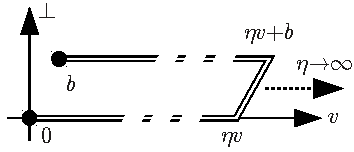
\includegraphics[width=0.5\linewidth]{figures/StapleLink2.pdf}
    \caption{Staple-shaped gauge link as in SIDIS and DY, following Ref.~\cite{Musch:2011er}.}
    \label{fig:staple}
\end{figure}

In Fig. \ref{fig:staple}, the two parallel Wilson lines are connected at the far end by another straight Wilson line. The complete gauge link thus has a staple-like shape. The vector $v$ sets the staple direction, and $\eta$ sets its extent. Lattice calculations are typically performed without any gauge fixing. We therefore prefer the notation with an explicitly gauge-invariant operator. Moreover, we compute at several finite staple extents $\eta$ (in lattice units, $\eta=0,\ldots,10$) and study the $\eta$ dependence. % TODO(Hari): the $\eta\to\infty$ limit belongs to the Results section (thesis Sec. 6). Even at finite $\eta$, this gauge-link geometry satisfies the desired symmetry transformation rules listed in Appendix~\ref{app:symmetries}. In this phenomenology frame, quark separation $b$ and staple extent $v$ are spacelike; in the lattice frame, however, they become purely spatial, as discussed in Sec.~\ref{sec:amplitudes_lattice}. 

The Lorentz-invariant Collins-Soper parameter, $\zeta \equiv 2 v \tcdot P/\sqrt{|v^2|}$, parameterizes the approach toward the physical light-like limit ($v = \nminus$). As $v$ becomes light-like, $\zeta \rightarrow \infty$; the parameter acts as an artificial scale that regulates the rapidity divergences~\cite{Collins:1981uk, Idilbi:2004vb, Aybat:2011ge}. Expressing the vectors $P$ and $v$ via rapidities $y_P$ and $y_v$ (we use $P^{\pm} = \mN e^{\pm y_P} / \sqrt{2}$ and $v^+/v^- = - e^{2y_v}$, with $v^->0$), we define the dimensionless variable:
\begin{equation}
	\hat \zeta \equiv \zeta / 2 \mN =  \frac{v \cdot P}{\sqrt{|v^2|} \sqrt{P^2}}=  \frac{v^+P^-+v^-P^+}{\sqrt{|v^2|} \mN} = \sinh(y_P - y_v)\ ,
	\label{eq-zeta}
\end{equation}
So $\hat \zeta$ measures the rapidity difference between the nucleon momentum and the Wilson line direction. This allows us to boost to a frame where $v$ is purely spatial ($v^0 = 0, y_v = 0$), which will be suited for lattice calculations.

\subsection{Amplitudes and the TMDs \texorpdfstring{$f_1$}{f1} and \texorpdfstring{$f_{1T}^\perp$}{f1Tperp}}
\label{sec:amplitudes_tmds}
The correlator $\widetilde\Phi^{[\gamma^\mu]}_\unsub$ is decomposed into Lorentz-invariant amplitudes $\tAmp_i$ and $\tBmp_i$, following Refs.~\cite{Musch:2011er,Goeke:2005hb}; the decomposition and the symmetry constraints on it are given in Appendix~\ref{app:symmetries}. In our frame ($b^+=0$, $\vprp{v}=\vprp{P}=0$), the kinematics fixes the relation between the invariants~\cite{MuschThesis2, Accardi:2009au}:
\begin{widetext}
\begin{align}
	\frac{v \tcdot b}{v \tcdot P} = b \tcdot P \frac{R(\zetahat^2)}{\mN^2}\, , \quad \text{where} \quad R(\zetahat^2) \equiv 1- \sqrt{1 + \hat \zeta^{-2}} = \frac{\mN^2}{v \tcdot P} \frac{v^+}{P^+} \, .
	\label{eq-lindeprel}
\end{align}
\end{widetext}
The relation in Eq. \eqref{eq-lindeprel} shows that the third argument of the $\tAmp_i$ and $\tBmp_i$ is not independent of the others in the context of TMDs.
Moreover, in our lattice calculations, we have to choose the link directions $b$ and $v$ such that Eq. \eqref{eq-lindeprel} is fulfilled. 
As a side remark, the parameter corresponding to Eq. \eqref{eq-lindeprel} in momentum space is $v \tcdot k / v \tcdot P \approx x$, i.e., the amplitudes $A_i$ and $B_i$ acquire an explicit $x$-dependence, which has already been pointed out in Refs.~\cite{MuschThesis2,Accardi:2009au}.
For the $\Gamma=\gamma^+$ structure at leading twist, the correlator can be written in the form 
\begin{align}
	\frac{1}{2 P^+}\widetilde \Phi^{[\gamma^+]}_{\unsub} & = 	
		\tAmp_{2B} 
		+ i \mN \epsilon_{ij} \vect{\bvec}_i \vect{S}_j\, \tAmp_{12B} \ ,
\end{align}
where the indices $i,j$ correspond to transverse directions, $i,j\in \{1,2\}$
(we use the convention $\epsilon^{0123}=1$ for the totally antisymmetric Levi-Civita symbol, and introduce $\myeps_{i j} \equiv \epsilon^{-+ij}$ such that $\myeps_{1 2} = 1$), and where we
have introduced the following abbreviations for combinations of amplitudes:
\begin{align}
	\tAmp_{2B}  & \ \equiv\  \tAmp_2 + R(\zetahat^2) \tBmp_1 \nonumber \displaybreak[0] \\
	\tAmp_{12B}  & \ \equiv\  \tAmp_{12} - R(\zetahat^2) \tBmp_8 \ . \displaybreak[0] 
	\label{eq-ABamps_sivers}
\end{align}
The unpolarized distribution $f_1$ and the Sivers distribution $f_{1T}^\perp$ follow from the Fourier integration operator $\fourint$:
\begin{widetext}
\begin{align}
	\fourint \tAmp_i \equiv & \int \frac{d^2 \vprp{\bvec}}{(2\pi)^2}\,e^{-i\vprp{\bvec}\tcdot\vprp{\kei}}\, \frac{1}{\widetilde{\mathcal{S}}(\bvec^2;\ldots)} \int \frac{d(\bvec \tcdot P)}{(2\pi)}\,e^{ix(\bvec \tcdot P)} 
	\tAmp_i(-\vprp{\bvec}^2,\bvec \tcdot P,(\bvec \tcdot P) R(\zetahat^2)/\mN^2,-1/(\mN\zetahat)^2,\eta v \tcdot P) \nonumber \\
	= & \int_0^\infty \frac{d(-\bvec^2)}{2(2\pi)}\ \frac{J_0(\sqrt{-\bvec^2}\, |\vprp{\kei}|)}{\widetilde{\mathcal{S}}(\bvec^2;\ldots)}\ \int \frac{d(\bvec \tcdot P)}{(2\pi)}\,e^{ix(\bvec \tcdot P)}\ 
	\tAmp_i(\bvec^2,\bvec \tcdot P,(\bvec \tcdot P) R(\zetahat^2)/\mN^2,-1/(\mN\zetahat)^2,\eta v \tcdot P) \, 
	\label{eq-fourint}
\end{align}
\end{widetext}
Applied to the combined amplitudes, it gives the leading-twist distributions:
\begin{align}
	 f_1(x,\vprp{\kei}^2;\zetahat,\ldots,\eta v \tcdot P) & = 2 \fourint\ \tAmp_{2B} \,,\nonumber \displaybreak[0] \\
	 f_{1T}^\perp(x,\vprp{\kei}^2;\zetahat,\ldots,\eta v \tcdot P) & =  4 m_N^2 \partial_{\vprp{\kei}^2} \fourint\ \tAmp_{12B} \ .
	 \label{eq-tmdsfromampsodd}
\end{align} 
Here, the dots ``$\ldots$'' indicate further parameters that specify the geometry of the soft factor. 
The $f_1$ is a T-even distribution which fulfills
\begin{align}
	f^{\text{T-even}}(x,\vprp{\kei}^2;\zetahat,\ldots,\eta v \tcdot P) = f^{\text{T-even}}(x,\vprp{\kei}^2;\zetahat,\ldots,-\eta v \tcdot P)
\end{align}
while the Sivers function $f_{1T}^\perp$ is a T-odd distribution which fulfills
\begin{align}
	f^{\text{T-odd}}(x,\vprp{\kei}^2;\zetahat,\ldots,\eta v \tcdot P) & = - f^{\text{T-odd}}(x,\vprp{\kei}^2;\zetahat,\ldots,-\eta v \tcdot P)
\end{align}
As a result, T-odd distributions must vanish for $\eta = 0$, which corresponds to straight gauge links.
TMDs for SIDIS and DY are obtained for $\eta v \tcdot P \rightarrow \infty$ and $\eta v \tcdot P \rightarrow -\infty$, respectively.
In the following, we choose $v \tcdot P \geq 0$, such that the SIDIS and DY limits for space-like $v$ can also be written as $\eta |v| \rightarrow \infty$ and $\eta |v| \rightarrow -\infty$, respectively.


Equation~\eqref{eq-tmdsfromampsodd} shows that the $x$-dependent TMDs in Fourier space, $\tilde f(x,\vprp{\bvec}^2)$ as defined in Eqs.~\eqref{eq-FTMD} and \eqref{eq-dFTMD}, are given directly by the Fourier transform of the amplitudes $\tAmp_{iB}$ with respect to $\bvec \tcdot P$.
For brevity, define the $x-(\bvec\tcdot P)$-Fourier-transformed, soft-factor-divided amplitudes
\begin{widetext}
\begin{equation}
	\tAmp^{[x]}_i(x,\vprp{\bvec}^2) \equiv \frac{1}{\widetilde{\mathcal{S}}(-\vprp{\bvec}^2;\ldots)} \int_{-\infty}^{\infty} \frac{d(\bvec \tcdot P)}{2\pi}\, e^{ix(\bvec \tcdot P)}\, \tAmp_{i}\big(-\vprp{\bvec}^2,\bvec \tcdot P,\ldots\big)\,,
\end{equation}
\end{widetext}
\begin{widetext}
\begin{align}
	\tilde f_1^{(0)}(x, \vprp{\bvec}^2;\zetahat,\ldots,\eta v \tcdot P) & = 2 \int_{-\infty}^{\infty} \frac{d(\bvec \tcdot P)}{2\pi}\, e^{ix(\bvec \tcdot P)}\, 
	\frac{\tAmp_{2B}\big(-\vprp{\bvec}^2,\bvec \tcdot P,(\bvec \tcdot P) R(\zetahat^2)/\mN^2,-1/(\mN\zetahat)^2,\eta v\tcdot P\big)}{\widetilde{\mathcal{S}}(-\vprp{\bvec}^2;\ldots)} \,,\displaybreak[0] \nonumber \\
    &=2\, \tAmp^{[x]}_{2B}(x,\vprp{\bvec}^2)\,. \label{eq-xintderfttmds1}\\
	\tilde f_{1T}^{\perp(1)}(x, \vprp{\bvec}^2;\zetahat,\ldots,\eta v \tcdot P) & = -2 \int_{-\infty}^{\infty} \frac{d(\bvec \tcdot P)}{2\pi}\, e^{ix(\bvec \tcdot P)}\, 
	\frac{\tAmp_{12B}\big(-\vprp{\bvec}^2,\bvec \tcdot P,(\bvec \tcdot P) R(\zetahat^2)/\mN^2,-1/(\mN\zetahat)^2,\eta v\tcdot P\big)}{\widetilde{\mathcal{S}}(-\vprp{\bvec}^2;\ldots)} \, ,\nonumber \\
    &=-2\,\tAmp^{[x]}_{12B}(x,\vprp{\bvec}^2)\,.
	\label{eq-xintderfttmds2}
\end{align}
\end{widetext}
We drop the soft-factor term from the definitions below, since it cancels in the ratios we consider.

\subsection{Generalized Sivers shift}
\label{sec:sivers_shift_amplitudes}
The derivation of Eqs.~\eqref{eq-xintderfttmds1} and~\eqref{eq-xintderfttmds2} is in Appendix~\ref{app:symmetries}; the arguments of the amplitudes are defined in Eq.~\eqref{eq-ab} there. Eqs. \eqref{eq-xintderfttmds1}-\eqref{eq-xintderfttmds2} identify $x$-dependent derivatives of Fourier-transformed TMDs with simple linear combinations of amplitudes $\tAmp_i$ and $\tBmp_i$ evaluated at the same values of $\vprp{\bvec}^2$, $\bvec \cdot P$, $\zetahat$ and $\eta v \tcdot P$. Forming ratios of these objects thus amounts to taking ratios of linear combinations of the fundamental correlators $\tilde \Phi^{[\Gamma]}_\unsub$ evaluated at the same point, i.e., with the same values of $\bvec$, $P$, and $\eta v$. For a discussion of the renormalization properties of ratios of the objects in \eqref{eq-xintderfttmds1}-\eqref{eq-xintderfttmds2}, it is thus sufficient to understand the renormalization properties of (ratios formed from) the correlators $\widetilde \Phi^{[\Gamma]}_\unsub = \frac{1}{2} \, \bra{P, S}\ \bar{q}(0)\, \Gamma\ \mathcal{U}\ q(\bvec)\ \ket{P, S} $.

As discussed in Refs.~\cite{Musch:2011er, Yoon:2017qzo}, analytical studies of the operator $\bar{q}(0)\, \Gamma\, \mathcal{U} q(\bvec)$ in the continuum suggest that for $\bvec^2 \neq 0$ the renormalization factors are multiplicative and $\Gamma$-independent. We will assume here that our lattice representation of $\bar{q}(0)\, \Gamma\, \mathcal{U}\, q(\bvec)$ is renormalized multiplicatively independent of $\Gamma$ as long as $|b|$ is larger than a few lattice spacings. % TODO(Hari): state the cut $|b|\ge 3a$ here and where the amplitudes are first shown (thesis Sec. 6) A more detailed discussion and numerical studies of this operator's renormalization properties appear in Ref.~\cite{Musch:2010ka}. Under the assumption of multiplicative renormalization, the soft factor and the renormalization factors cancel in ratios of amplitudes evaluated at the same $\bvec$, $P$ and $\eta v$, and such ratios depend only on $\vprp{\bvec}^2$, $P\cdot b$, $\zetahat$, and the staple extent $\eta v \tcdot P$.

From phenomenology, the Sivers shift is the ratio defined as
\begin{widetext}
\begin{align}
	\langle \vect{k}_y \rangle_{TU} \equiv \mN \frac{f_{1T}^{\perp(1)}(x)}{f_1^{(0)}(x)} = 
	\left. \frac{ \int d^2 \vprp{\kei}\, \vect{\kei}_y  \ \Phi^{[\gamma^+]}(x,\vprp{\kei},P,S;\ldots) }{ \int d^2 \vprp{\kei}  \phantom{\vect{\kei}_y}\ \Phi^{[\gamma^+]}(x,\vprp{\kei},P,S;\ldots) } \right|_{\displaystyle \vprp{S}=(1,0) }\, , \label{eq-sivshift}
\end{align}
\end{widetext}
where $\gamma^+$ projects onto the leading twist.
The ratio above yields the average transverse momentum
in the $y$-direction, for quarks with a given longitudinal momentum fraction $x$ inside a proton polarized in the $x$-direction. As mentioned before, understanding $f_{1T}^{\perp(1)}$ simply as a $\vprp{\kei}$-weighted TMD is problematic, since the $\vprp{k}$-integral is expected to be UV divergent. 
A natural way of circumventing this divergence is to generalize the Sivers shift to an expression in terms of the Fourier-transformed TMDs:
\begin{widetext}
\begin{align}
    \langle \vect{k}_y \rangle_{TU}(\vprp{\bvec}^2,x,\zetahat,\eta v \tcdot P) 
	&\ \equiv\ \mN \frac{\tilde f_{1T}^{\perp(1)}(\vprp{\bvec}^2,x;\zetahat,\ldots,\eta v \tcdot P)}{\tilde f_1^{(0)}(\vprp{\bvec}^2,x;\zetahat,\ldots,\eta v \tcdot P)}  \\
 &=-m_{N} \frac{\int d(b\cdot P)e^{ix(b\cdot P)} \tAmp_{12B}(\bvec^2,\bvec \tcdot P,(\bvec \tcdot P) R(\zetahat^2)/\mN^2,-1/(\mN\zetahat)^2,\eta v \tcdot P)}{\int d(b\cdot P)e^{ix(b\cdot P)}\tAmp_{2B}(\bvec^2,\bvec \tcdot P,(\bvec \tcdot P) R(\zetahat^2)/\mN^2,-1/(\mN\zetahat)^2,\eta v \tcdot P)} \\
 &\ \xrightarrow{\vprp{\bvec}^2 = 0} 
		\left. \frac{  \int d^2 \vprp{\kei}\, \vect{\kei}_y  \ \Phi^{[\gamma^+]}(x,\vprp{\kei},P,S;\ldots) }
		{  \int d^2 \vprp{\kei}  \phantom{\vect{\kei}_y}\ \Phi^{[\gamma^+]}(x,\vprp{\kei},P,S;\ldots) } \right|_{\displaystyle \vprp{S}=(1,0) } 
	\label{eq-genSivShift}
\end{align}
\end{widetext}
In the limit $\vprp{\bvec}^2=0$ we recover the Sivers shift \eqref{eq-sivshift}, because the Fourier transformed TMDs $\tilde f_{1T}^{\perp(1)}$ and $\tilde f_1^{(0)}$ coincide with the moments $f_{1T}^{\perp(1)}$ and $f_1^{(0)}$, respectively. However, we are interested in the generalized Sivers shift for non-zero $\vprp{\bvec}^2$, where this UV divergence disappears. The variable $\vprp{b}^2$ effectively acts as a regulator. Moreover, the $\vprp{\bvec}$-dependence allows us to study differences in the widths of distributions on a qualitative level.

Furthermore, the generalized Sivers shift is T-odd, i.e., we expect to obtain results of opposite sign in the SIDIS and DY limits $\eta v \tcdot P \rightarrow \infty$ and $\eta v \tcdot P \rightarrow -\infty$, respectively, as demonstrated in Refs.~\cite{Musch:2011er,Yoon:2017qzo}.

In summary, the generalized Sivers shift describes a feature of the transverse momentum distribution of (unpolarized) quarks in a transversely polarized proton. In the formal limit $\vprp{\bvec}^2 = 0$, it measures the dipole moment of that distribution orthogonal to the polarization of the proton.
